\section{CHAPTER 5: PRODUCTION}

\subsection{Overview:}

In the production section there is Dyeing, Knitting, Printing and Washing. There
was a soft flow machine for dyeing which produces 30 tons of products in
a day. There was a Slitting machine to make the round fabric into an
open form. Then there was a stenter machine for the dryer and heat
setting of the fabric. Thermic Oil used for stenter. There was a
Compacting machine as well for fabric shrinkage control. There were also
knitting machines producing 25 tons of products in a day. Fabric made in
a round shape here. This fabric is called Greig Fabric. The printing
machine was screen print type and 50 tons of products can be printed per
day. There were several washing machines whose capacity was 2000 per
day.


\subsection{Dyeing Machine:}

A soft flow dyeing machine is a textile processing device used in the
dyeing of fabrics, primarily made from natural or synthetic fibers.

\subsubsection{Description:}


Soft flow dyeing machines are designed to provide a gentle and uniform
dyeing process for delicate fabrics, ensuring minimal damage or
creasing. They operate by circulating a dye liquor through the fabric in
a controlled manner, allowing for even penetration of the dye solution
into the fibers.


\subsubsection{Functionality:}

\begin{enumerate}
\item
  Fabric Loading: Fabrics are loaded into the dyeing machine, either in
  loose form or on perforated rollers, to ensure even dye distribution.
\item
  Dye Liquor Circulation: The dye liquor, consisting of water, dye, and
  auxiliary chemicals, is circulated through the fabric using a
  combination of pumps, nozzles, and a specially designed flow system.
\item
  Temperature and Pressure Control: Soft flow dyeing machines maintain
  precise control over temperature and pressure parameters to ensure
  optimal dyeing conditions for different types of fabrics and dyes.
\item
  Dyeing Cycle: The dyeing process typically involves multiple cycles of
  dyeing, rinsing, and draining to achieve the desired color depth and
  uniformity.
\item
  Versatility: Soft flow dyeing machines are suitable for a wide range
  of fabrics, including cotton, polyester, wool, and blends, making them
  versatile for various textile applications.
\end{enumerate}

\subsubsection{Advantages:}

\begin{enumerate}
\item
  Gentle Treatment: Soft flow dyeing machines provide gentle treatment
  of fabrics, minimizing damage, creasing, and distortion during the
  dyeing process.
\item
  Even Dye Penetration: The controlled flow of dye liquor ensures even
  penetration of the dye solution into the fabric, resulting in uniform
  coloration and consistent dyeing results.
\item
  Reduced Water and Chemical Consumption: These machines are designed to
  optimize dye liquor circulation, leading to reduced water and chemical
  consumption compared to traditional dyeing methods.
\item
  Energy Efficiency: Soft flow dyeing machines incorporate
  energy-efficient features such as temperature control systems and
  optimized flow dynamics, contributing to lower energy consumption
  during the dyeing process.
\end{enumerate}

\subsubsection{Disadvantages:}

\begin{enumerate}
\item
  High Initial Cost: Soft flow dyeing machines typically involve a
  significant initial investment due to their sophisticated design and
  advanced technology.
\item
  Maintenance Requirements: Regular maintenance and servicing are
  necessary to ensure the optimal performance of soft flow dyeing
  machines, which may incur additional costs and downtime.
\item
  Limited Capacity: Depending on the size and configuration, soft flow
  dyeing machines may have limited capacity compared to other dyeing
  equipment, which could impact production throughput.
\end{enumerate}

\subsection{Slitting Machine:}


A slitting machine, also known as a slitter or slitting line, is a piece
of industrial equipment used to cut large rolls or coils of material
into narrower strips.

\begin{figure}[h!]
  \centering
  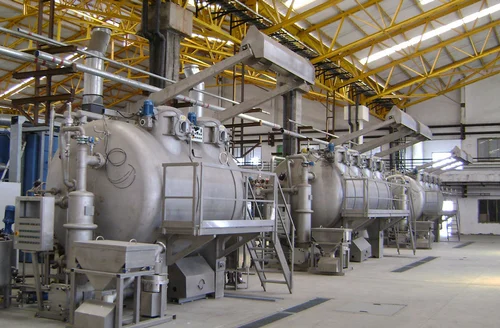
\includegraphics[width=0.7\linewidth]{figs/production/image1.png}
  \caption{Dyeing Machine}
  \label{fig:Dyeing Machine}
\end{figure}

\begin{figure}[h!]
  \centering
  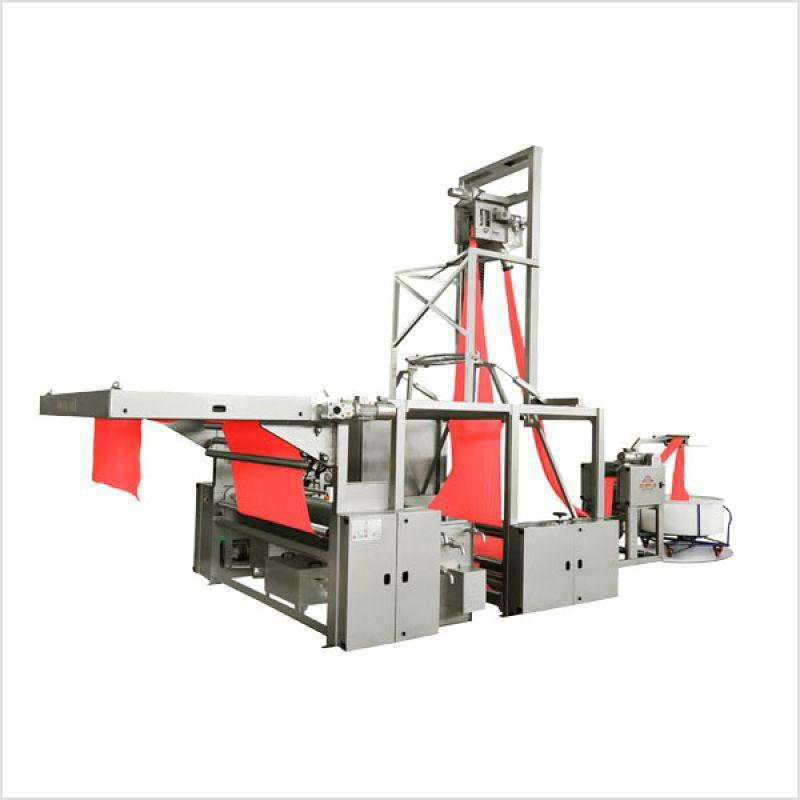
\includegraphics[width=0.7\linewidth]{figs/production/image2.jpg}
  \caption{Slitting Machine}
  \label{fig:Slitting Machine}
\end{figure}


\subsubsection{Description:}

A slitting machine typically consists of several components, including:

\begin{enumerate}
\item
  Unwinder: Where the large roll or coil of material is loaded for
  processing.
\item
  Slitting knives or blades: These are used to cut the material into
  narrower strips.
\item
  Rewinder: Where the slit strips are rewound into smaller coils or
  spools.
\item
  Tension control system: Ensures proper tension is maintained on the
  material throughout the slitting process.
\item
  Control panel: Allows operators to adjust settings such as cutting
  width, speed, and tension.
\end{enumerate}

\subsubsection{Functionality:}

\begin{enumerate}
\item
  Material feeding: The roll or coil of material is loaded onto the
  unwinder and fed into the slitting machine.
\item
  Slitting: The material passes through the slitting knives or blades,
  which cut it into narrower strips. The number of blades and their
  spacing determine the width of the strips.
\item
  Rewinding: The slit strips are rewound onto individual cores or spools
  on the rewinder.
\item
  Quality control: Operators monitor the slitting process to ensure the
  strips are cut accurately and without defects.
\end{enumerate}

\subsubsection{Advantages:}

\begin{enumerate}
\item
  Customization: Slitting machines allow manufacturers to produce strips
  of varying widths and lengths, catering to different customer
  requirements.
\item
  Efficiency: Slitting machines can process large rolls or coils of
  material quickly and efficiently, increasing productivity.
\item
  Versatility: Slitting machines can handle a wide range of materials,
  including metal, plastic, paper, film, and textiles, making them
  suitable for various industries.
\end{enumerate}

\subsubsection{Disadvantages:}

\begin{enumerate}
\item
  Initial investment: Slitting machines can be expensive to purchase and
  install, especially for larger or more advanced models.
\item
  Maintenance: Regular maintenance is required to keep slitting machines
  in optimal working condition, including sharpening blades, replacing
  worn parts, and calibrating tension control systems.
\item
  Complexity: Operating slitting machines may require specialized
  training and expertise, particularly when dealing with different
  materials or adjusting settings for specific requirements.
\end{enumerate}

\subsection{Stenter Machine:}


A stenter machine is a textile finishing machine used to apply various
treatments and finishes to fabrics.


\subsubsection{Description:}


A stenter machine typically consists of the following main components:


\begin{enumerate}
\item
  Entry and exit sections: Where the fabric enters and exits the
  machine.
\item
  Tentering chains: Continuous chains with clips or pins that hold the
  fabric edges taut and straight throughout the process.
\item
  Frame: Supports the tentering chains and other components of the
  machine.
\item
  Heating chambers: Where the fabric is subjected to heat to remove
  moisture and apply treatments or finishes.
\item
  Air circulation system: Ensures even distribution of heat and airflow
  across the fabric.
\end{enumerate}

\subsubsection{Functionality:}

\begin{enumerate}
\item
  Fabric feeding: The fabric is fed into the stenter machine from a roll
  or other source.
\item
  Tentering: The fabric is held taut and straight by the tentering
  chains, which stretch it to the desired width.
\item
  Heat treatment: The fabric passes through heating chambers, where it
  is subjected to controlled temperatures to remove moisture and apply
  treatments such as drying, curing, or coating.
\item
  Cooling: After heat treatment, the fabric may pass through cooling
  chambers to reduce its temperature and stabilize the applied
  treatments.
\item
  Finishing: Additional processes such as brushing, shearing, or
  calendering may be performed to achieve specific surface textures or
  finishes.
\item
  Fabric winding: The finished fabric is wound onto a roll or other
  suitable form for further processing or packaging.
\end{enumerate}

\subsubsection{Advantages:}

\begin{enumerate}
\item
  Uniform treatment: Stenter machines provide uniform application of
  treatments and finishes across the entire width of the fabric,
  ensuring consistent quality and appearance.
\item
  Controlled process: The stentering process can be precisely
  controlled, allowing for adjustments to temperature, humidity, and
  other parameters to achieve desired results.
\item
  Increased productivity: Stenter machines can handle large volumes of
  fabric efficiently, making them suitable for high-volume production in
  textile finishing operations.
\end{enumerate}

\subsubsection{Disadvantages:}

\begin{enumerate}
\item
  Initial investment: Stenter machines can be expensive to purchase and
  install, especially for larger or more advanced models.
\item
  Energy consumption: The heating and drying processes used in stenter
  machines require significant energy input, leading to higher operating
  costs.
\item
  Maintenance: Regular maintenance is required to keep stenter machines
  in optimal working condition, including cleaning, lubrication, and
  replacement of worn parts.
\end{enumerate}

\subsection{Compacting Machine:}


A compacting machine, also known as a compactor or felt compacting
machine, is a textile processing device used to improve the properties
of fabric, particularly knitted fabrics.


\subsubsection{Description:}


A compacting machine typically consists of the following main
components:


\begin{enumerate}
\item
  Entry and exit sections: Where the fabric enters and exits the
  machine.
\end{enumerate}

\begin{figure}[h!]
  \centering
  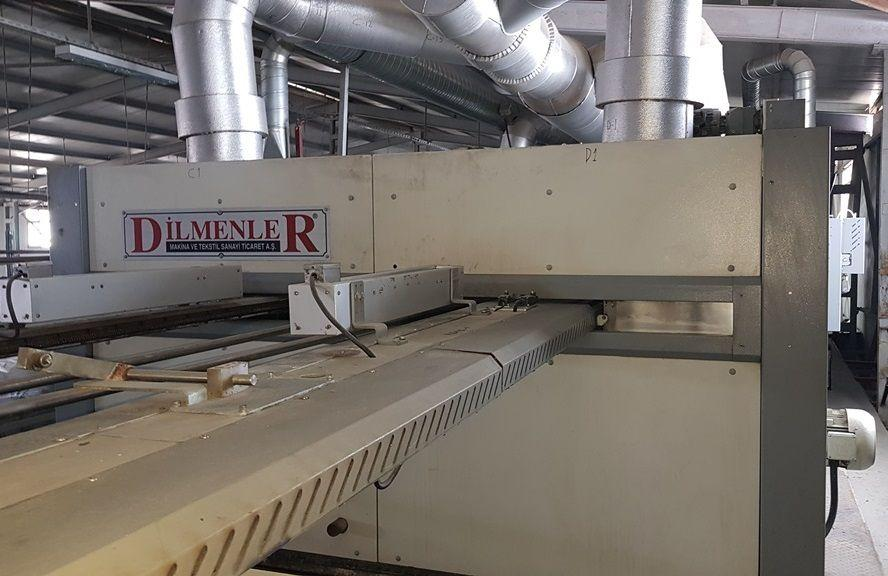
\includegraphics[width=0.7\linewidth]{figs/production/image3.jpg}
  \caption{Stenter Machine}
  \label{fig:Stenter Machine}
\end{figure}


\begin{figure}[h!]
  \centering
  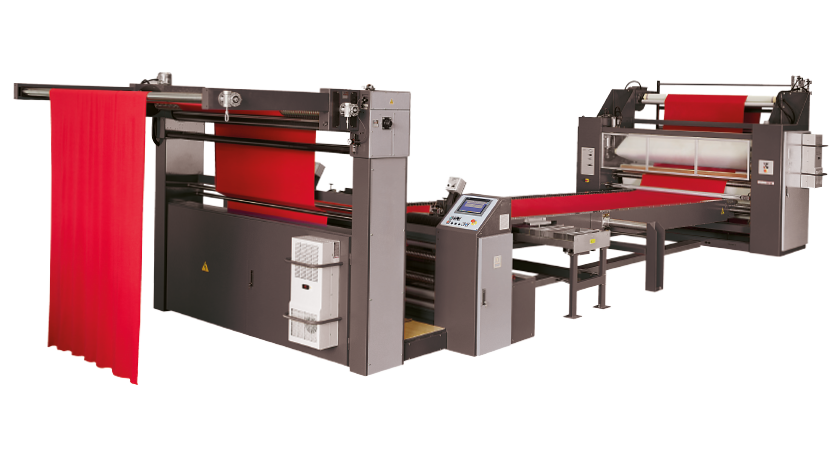
\includegraphics[width=0.7\linewidth]{figs/production/image4.png}
  \caption{Compacting Machine.}
  \label{fig:Compacting Machine.}
\end{figure}


\begin{enumerate}
\item
  Compacting rollers: These rollers compress the fabric, reducing its
  thickness and improving its dimensional stability.
\item
  Tension control system: Ensures proper tension is maintained on the
  fabric throughout the compacting process.
\item
  Heating system (optional): Some compacting machines may include a
  heating system to soften the fabric fibers, allowing for better
  compression.
\end{enumerate}

\subsubsection{Functionality:}

\begin{enumerate}
\item
  Fabric feeding: The fabric is fed into the compacting machine from a
  roll or other source.
\item
  Compression: As the fabric passes through the compacting rollers, it
  is subjected to pressure, which compresses the fibers and reduces the
  thickness of the fabric.
\item
  Heat treatment (optional): In some cases, the fabric may be subjected
  to heat during the compacting process to soften the fibers and enhance
  the compression effect.
\item
  Cooling: After compression, the fabric may pass through cooling
  chambers to reduce its temperature and stabilize its properties.
\item
  Fabric winding: The compacted fabric is wound onto a roll or other
  suitable form for further processing or packaging.
\end{enumerate}

\subsubsection{Advantages:}

\begin{enumerate}
\item
  Improved fabric properties: Compact machines can improve the
  dimensional stability, smoothness, and appearance of fabrics by
  compressing the fibers and reducing shrinkage.
\item
  Increased fabric density: The compression process increases the
  density of the fabric, making it more resistant to stretching and
  deformation.
\item
  Enhanced fabric performance: Compact fabrics exhibit better resistance
  to pilling, wrinkling, and creasing, resulting in higher-quality end
  products.
\end{enumerate}


Disadvantages:


\begin{enumerate}
\item
  Initial investment: Compact machines can be expensive to purchase and
  install, especially for larger or more advanced models.
\item
  Energy consumption: The compression and heat treatment processes used
  in compacting machines require significant energy input, leading to
  higher operating costs.
\item
  Maintenance: Regular maintenance is required to keep compacting
  machines in optimal working condition, including cleaning,
  lubrication, and replacement of worn parts.
\end{enumerate}

\subsection{Knitting Machine:}


A knitting machine is a piece of textile manufacturing equipment used to
produce knitted fabrics from yarn.


\subsubsection{Description:}


Knitting machines come in various types, including flatbed, circular,
and warp knitting machines. They consist of a needle bed, yarn feeders,
carriage or cam system, and controls for adjusting stitch size and
pattern.


\subsubsection{Functionality:}

\begin{enumerate}
\item
  Yarn Feeding: Yarn is fed into the machine from multiple feeders or
  cones, depending on the type of knitting machine.
\item
  Stitch Formation: Needles or hooks on the machine interlock the yarn
  to form loops or stitches, creating the fabric.
\item
  Fabric Formation: The carriage or cam system moves across the needle
  bed, manipulating the needles to form rows of stitches and build up
  the fabric.
\item
  Control: Knitting machines may have controls for adjusting stitch
  size, tension, and pattern to create different textures, designs, and
  structures.
\end{enumerate}

\subsubsection{Advantages:}

\begin{enumerate}
\item
  Versatility: Knitting machines can produce a wide range of fabrics,
  including jerseys, rib knits, and jacquards, with various textures,
  patterns, and thicknesses.
\item
  Efficiency: Knitting machines can achieve high production speeds,
  making them suitable for mass production of knitted garments,
  textiles, and accessories.
\item
  Customization: Knitting machines offer flexibility in design and
  customization, allowing for the creation of unique and personalized
  knitted products.
\end{enumerate}

\subsubsection{Disadvantages:}

\begin{enumerate}
\item
  Complexity: Operating and maintaining knitting machines require
  specialized skills and knowledge. Troubleshooting and repairing
  technical issues can be challenging.
\item
  Cost: Knitting machines can be expensive to purchase and maintain,
  especially advanced models with computerized controls and features.
\item
  Fabric Limitations: Knitting machines may have limitations in terms of
  fabric width, gauge, and complexity, restricting the types of fabrics
  and designs that can be produced.
\end{enumerate}

\begin{figure}[h!]
  \centering
  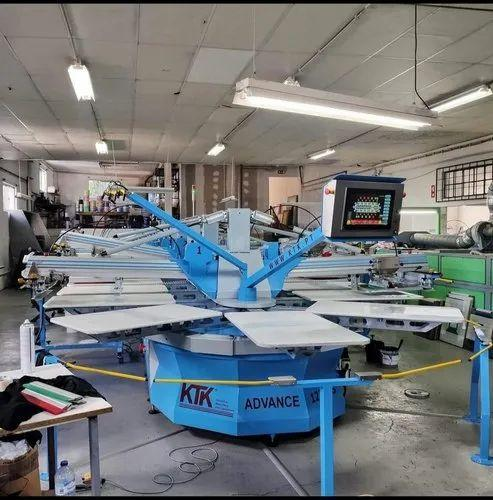
\includegraphics[width=0.7\linewidth]{figs/production/image5.jpg}
  \caption{Knitting Machine}
  \label{fig:Knitting Machine}
\end{figure}

\begin{figure}[h!]
  \centering
  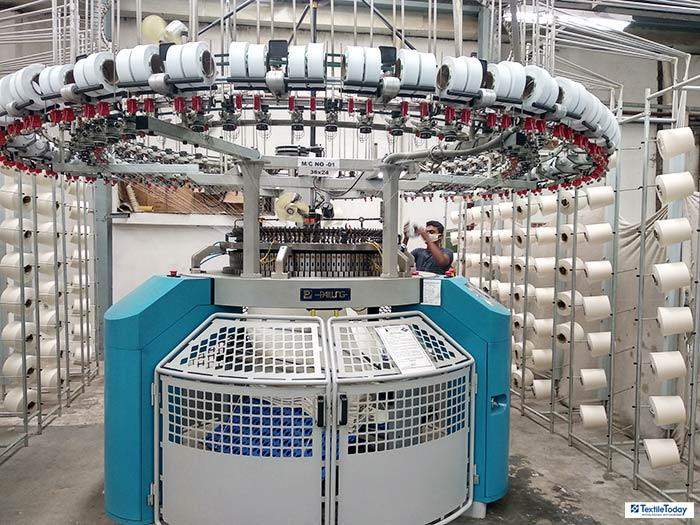
\includegraphics[width=0.7\linewidth]{figs/production/image6.jpg}
  \caption{Printing Machine}
  \label{fig:Printing Machine}
\end{figure}


\subsection{Printing Machine:} A screen printing machine, also known
as a silk screen printing machine or serigraph machine, is a printing
device used to apply ink onto various substrates, including textiles,
paper, plastics, glass, and metals.

\subsubsection{Description:}


A screen printing machine typically consists of the following main
components:


\begin{enumerate}
\item
  Screen frame: A frame made of wood, aluminum, or steel, with a
  stretched mesh screen tightly attached.
\item
  Squeegee: A rubber or plastic blade used to push ink through the mesh
  screen onto the substrate.
\item
  Printing bed: The surface where the substrate is placed for printing.
\item
  Registration system: Guides or stops to ensure accurate alignment of
  the substrate for multiple-color printing.
\item
  Ink reservoir: A container for holding the printing ink, typically
  located above the screen frame.
\end{enumerate}

\subsubsection{Functionality:}

\begin{enumerate}
\item
  Preparation: The design to be printed is first transferred onto a
  stencil or mesh screen using a photographic process or manually
  applied emulsion.
\item
  Setup: The substrate is placed onto the printing bed, and the screen
  frame is positioned over it.
\item
  Ink application: Ink is poured onto the screen frame, and a squeegee
  is used to spread the ink evenly across the screen.
\item
  Printing: The squeegee is then pulled across the screen, forcing the
  ink through the mesh and onto the substrate, creating the desired
  design or pattern.
\item
  Curing: After printing, the substrate may pass through a curing or
  drying process, typically involving heat or UV light, to set the ink
  and ensure durability.
\end{enumerate}

\subsubsection{Advantages:}

\begin{enumerate}
\item
  Versatility: Screen printing machines can be used to print on
  textiles, paper, plastics, and more.
\item
  Durability: Screen-printed designs are highly durable and resistant to
  fading, making them suitable for outdoor use and long-lasting
  applications.
\item
  High-quality prints: Screen printing allows for precise control over
  ink thickness and color saturation, resulting in vibrant and detailed
  prints.
\item
  Cost-effectiveness: Screen printing is a cost-effective method for
  producing medium to large quantities of printed materials, especially
  for multicolor designs.
\end{enumerate}

\subsubsection{Disadvantages:}

\begin{enumerate}
\item
  Setup time: Setting up a screen printing machine can be
  time-consuming, especially for complex designs or multiple-color
  prints.
\item
  Limited color options: Screen printing is best suited for designs with
  fewer colors, as each color requires a separate screen and setup.
\item
  Not suitable for small runs: Screen printing is not cost-effective for
  small print runs due to setup costs and time.
\item
  Skill required: Achieving consistent and high-quality prints with
  screen printing requires skill and experience, particularly in screen
  preparation and ink application.
\end{enumerate}

